\documentclass[11pt]{article}
\usepackage[utf8]{inputenc}
\usepackage[dvips]{graphicx}
\usepackage{fancybox}
\usepackage{verbatim}
\usepackage{array}
\usepackage{latexsym}
\usepackage{alltt}
\usepackage{hyperref}
\usepackage{textcomp}
\usepackage{color}
\usepackage{amsmath}
\usepackage{amsfonts}
\usepackage{tikz}
\usepackage{float}
\usepackage[hmargin=3cm,vmargin=5.0cm]{geometry}
%\topmargin=0cm
\topmargin=-2cm
\addtolength{\textheight}{6.5cm}
\addtolength{\textwidth}{2.0cm}
%\setlength{\leftmargin}{-5cm}
\setlength{\oddsidemargin}{0.0cm}
\setlength{\evensidemargin}{0.0cm}


\begin{document}

\section*{Student Information } 
%Write your full name and id number between the colon and newline
%Put one empty space character after colon and before newline
Full Name : Mustafa Ozan ALPAY \\
Id Number : 2309615 \\

% Write your answers below the section tags
\section*{Answer 1}
$$ S= \{``",``1",``0",``10",``01",``010",``011",``101",``110" \}$$ 
\subsection*{a}  

\begin{figure}[H]
	\centering
	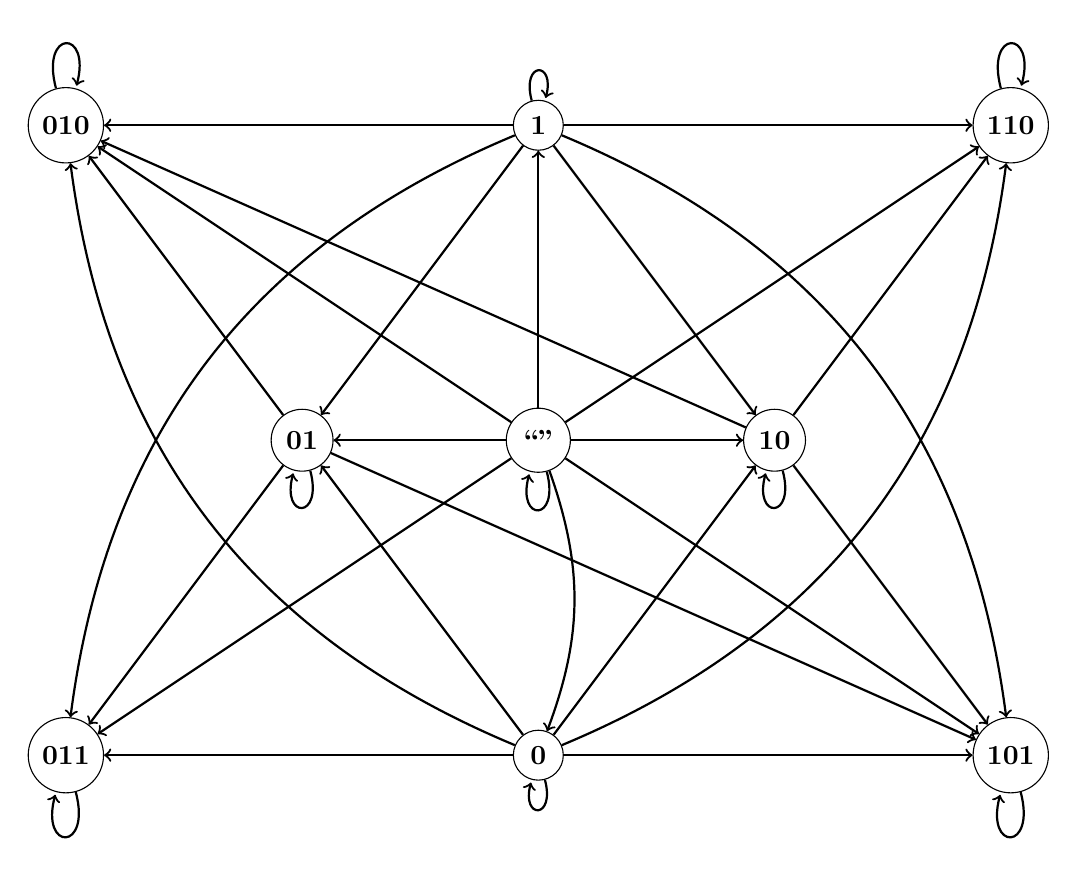
\begin{tikzpicture}
	
	\node[shape=circle,draw=black] (d) at (3, 4)     {\textbf{01}};
	\node[shape=circle,draw=black] (b) at (6, 8)     {\textbf{1}};
	\node[shape=circle,draw=black] (e) at (6, 4)     {\textbf{``"}};
	\node[shape=circle,draw=black] (h) at (6, 0)     {\textbf{0}};
	\node[shape=circle,draw=black] (g) at (0, 0)     {\textbf{011}};
	\node[shape=circle,draw=black] (f) at (9, 4)     {\textbf{10}};
	\node[shape=circle,draw=black] (c) at (12, 8)     {\textbf{110}};
	\node[shape=circle,draw=black] (i) at (12, 0)     {\textbf{101}};
	\node[shape=circle,draw=black] (a) at (0, 8)     {\textbf{010}};
	
    \path[->, thick] (a) edge [loop above] (a);
    \path[->, thick] (b) edge [loop above] (b);
    \path[->, thick] (c) edge [loop above] (c);
    \path[->, thick] (d) edge [loop below] (d);
    \path[->, thick] (e) edge [loop below] (e);
    \path[->, thick] (f) edge [loop below] (f);
    \path[->, thick] (g) edge [loop below] (g);
    \path[->, thick] (h) edge [loop below] (h);
    \path[->, thick] (i) edge [loop below] (i);
    
    \path[->, thick] (e) edge (a);
    \path[->, thick] (e) edge (b);
    \path[->, thick] (e) edge (c);
    \path[->, thick] (e) edge (d);
    \path[->, thick] (e) edge (f);
    \path[->, thick] (e) edge (g);
    \path[->, thick] (e) edge [bend left=20] (h);
    \path[->, thick] (e) edge (i);
    
    \path[->, thick] (b) edge (a);
    \path[->, thick] (b) edge (c);
    \path[->, thick] (b) edge (d);
    \path[->, thick] (b) edge (f);
    \path[->, thick] (b) edge [bend right=30] (g);
    \path[->, thick] (b) edge [bend left=30] (i);
    
    \path[->, thick] (h) edge [bend left=30] (a);
    \path[->, thick] (h) edge [bend right=30] (c);
    \path[->, thick] (h) edge (d);
    \path[->, thick] (h) edge (f);
    \path[->, thick] (h) edge (g);
    \path[->, thick] (h) edge (i);
    
    \path[->, thick] (d) edge (a);
    \path[->, thick] (d) edge (g);
    \path[->, thick] (d) edge (i);
    
    \path[->, thick] (f) edge (a);
    \path[->, thick] (f) edge (c);
    \path[->, thick] (f) edge (i);

	\end{tikzpicture} 
	\caption{R in Q1, as a directed graph.}	
	\label{rdg1}
\end{figure}

\subsection*{b}
\begin{itemize}
    \item  \textbf{Definition 1} from the Section 9.6 of the textbook says that 
    \begin{quote}
        A relation $R$ on a set $S$ is called a partial ordering if it is reflexive, antisymmetric, and transitive. A set $S$ together with a partial ordering R is called a poset.
    \end{quote}
    Therefore, we need to prove that Graph \ref{rdg1} is reflexive, antisymmetric, and transitive.
    \item \textbf{Reflexivity}: Since each element has a loop to itself, the graph is reflexive.
    \item \textbf{Antisymmetry}: Since there are no two edges between two vertices with different directions, the graph is antisymmetric.
    \item \textbf{Transitivity}: By looking at the graph, we can see that vertices $1,0,01,10$ have edges to and from them. Investigating these vertices should be enough to determine if the graph is transitive.
    \begin{itemize}
        \item Vertex 01 has 3 incoming edges: ``", 0, and 1. When we look at the outgoing edges of vertex 01, we can see that 010, 011, and 101 also have incoming edges from Vertex 01's incoming edges. 
        \item Similarly, Vertex 10 has 3 incoming edges: ``", 0, and 1. When we look at the outgoing edges of Vertex 01, we can see that 010, 101, and 110 also have incoming edges from Vertex 10's incoming edges. 
        \item Vertex 1 has 1 incoming edge: ``". When we look at the outgoing edges of Vertex 1, we can see that 010, 01, 011, 10, 101, and 110 also have incoming edges from Vertex 1's incoming edge. 
        \item Similarly, Vertex 0 has 1 incoming edge: ``". When we look at the outgoing edges of Vertex 0, we can see that 010, 01, 011, 10, 101, and 110 also have incoming edges from Vertex 0's incoming edge. 
    \end{itemize}
    \item Since we have shown that that Graph \ref{rdg1} is reflexive, antisymmetric, and transitive, the partial ordering $(S,R)$ is a poset.
\end{itemize}

\subsection*{c}
\begin{itemize}
    \item  \textbf{Definition 3} from the Section 9.6 of the textbook says that 
    \begin{quote}
        If $(S, \propto) $ is a poset and every two elements of $S$ are comparable, $S$ is called a totally ordered set, and $\propto$ is called a total order.
    \end{quote}
    \item Since $(S,R)$ is a poset, and since each member of $S$ is a string, thus comparable, $S$ is a totally ordered set, and $R$ is a total order.
\end{itemize}

\subsection*{d}

\begin{figure}[H]
	\centering
	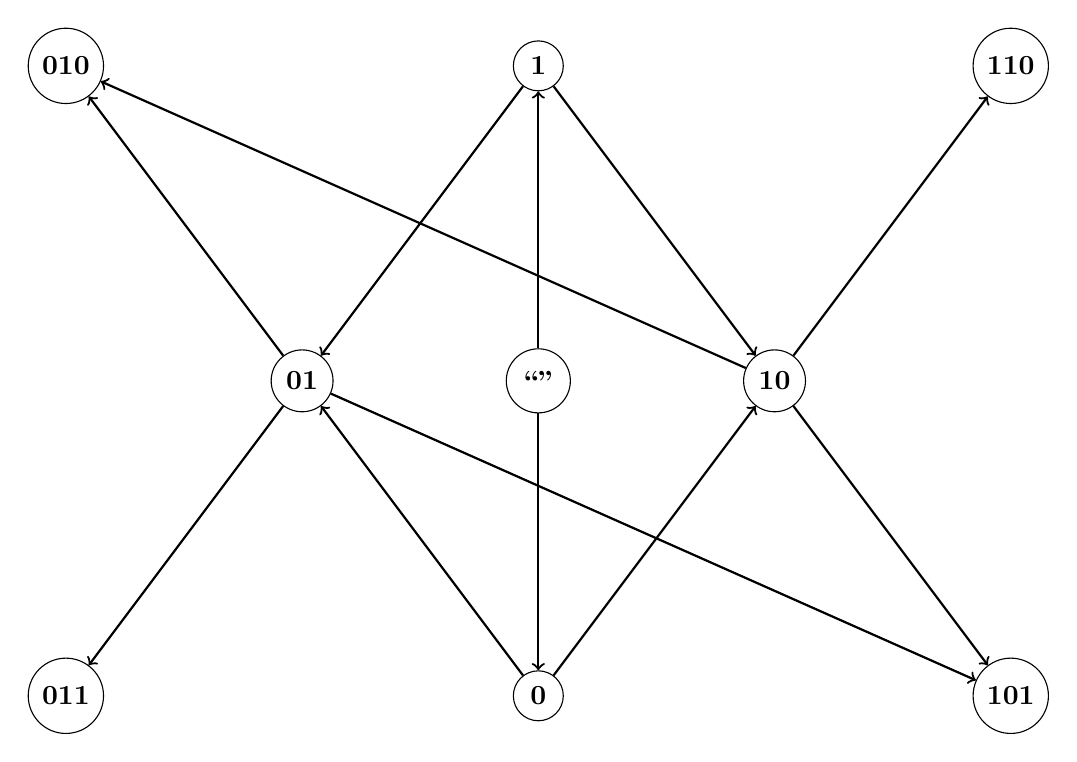
\begin{tikzpicture}
	
	\node[shape=circle,draw=black] (d) at (3, 4)     {\textbf{01}};
	\node[shape=circle,draw=black] (b) at (6, 8)     {\textbf{1}};
	\node[shape=circle,draw=black] (e) at (6, 4)     {\textbf{``"}};
	\node[shape=circle,draw=black] (h) at (6, 0)     {\textbf{0}};
	\node[shape=circle,draw=black] (g) at (0, 0)     {\textbf{011}};
	\node[shape=circle,draw=black] (f) at (9, 4)     {\textbf{10}};
	\node[shape=circle,draw=black] (c) at (12, 8)     {\textbf{110}};
	\node[shape=circle,draw=black] (i) at (12, 0)     {\textbf{101}};
	\node[shape=circle,draw=black] (a) at (0, 8)     {\textbf{010}};

    
    \path[->, thick] (e) edge (b);
    \path[->, thick] (e) edge (h);
    
    \path[->, thick] (b) edge (d);
    \path[->, thick] (b) edge (f);

    \path[->, thick] (h) edge (d);
    \path[->, thick] (h) edge (f);
    
    \path[->, thick] (d) edge (a);
    \path[->, thick] (d) edge (g);
    \path[->, thick] (d) edge (i);
    
    \path[->, thick] (f) edge (c);
    \path[->, thick] (f) edge (i);
    \path[->, thick] (f) edge (a);

	\end{tikzpicture} 
	\caption{(S,R) as a Hasse Diagram.}	
	\label{rdg4}
\end{figure}
\pagebreak
\subsection*{e}

\begin{itemize}
    \item The Lattice definition from the Section 9.6 of the textbook says that 
    \begin{quote}
        A partially ordered set in which every pair of elements has both a least upper bound and a greatest lower bound is called a lattice.
    \end{quote}
    \item Let us pick 011 and 10. When we look at the Hasse Diagram in Figure \ref{rdg4}, we can clearly see that they have two great lower bounds, namely 0 and 1. However when we try to find a least upper bound, we can see that it does not exist. 
    \item Therefore, the Hasse Diagram in Figure \ref{rdg4} is not a lattice.
\end{itemize}


\section*{Answer 2}
\subsection*{a}

\begin{table}[H]
    \centering
    \begin{tabular}{|c|c|}	
    \hline 							
    \textbf{Initial Vertex} & \textbf{Terminal Vertices}  \\
    \hline 
    \hline 
    a & a, b, d \\ \hline
    b & c, d \\ \hline
    c & b \\ \hline
    d & c \\ \hline
    e & b, f \\ \hline
    f & b, e, f \\ \hline
    g & c, f \\ \hline
    \end{tabular}
    \caption{ Adjacency List for Graph G in Q2 }
    \end{table}

\subsection*{b}
\begin{figure}[H]
$$  \begin{bmatrix}
        1 & 1 & 0 & 1 & 0 & 0 & 0 \\
        0 & 0 & 1 & 1 & 0 & 0 & 0 \\
        0 & 1 & 0 & 0 & 0 & 0 & 0 \\
        0 & 0 & 1 & 0 & 0 & 0 & 0 \\
        0 & 1 & 0 & 0 & 0 & 1 & 0 \\
        0 & 1 & 0 & 0 & 1 & 1 & 0 \\
        0 & 0 & 1 & 0 & 0 & 1 & 0 \\
    \end{bmatrix} $$
    \caption{Adjacency Matrix for Graph G in Q2}
\end{figure}

\subsection*{c}
\begin{table}[H]
    \centering
    \begin{tabular}{|c|c|c|}	
    \hline 							
    & \textbf{In-degrees Count} & \textbf{Out-degrees Count}  \\
    \hline 
    \hline 
    a & 1 & 3 \\ \hline
    b & 4 & 2 \\ \hline
    c & 3 & 1 \\ \hline
    d & 2 & 1 \\ \hline
    e & 1 & 2 \\ \hline
    f & 3 & 3 \\ \hline
    g & 0 & 2 \\ \hline
    \end{tabular}
    \caption{ In-degrees and Out-degrees of every vertex of Graph G in Q2 }
    \end{table}

\subsection*{d}
\begin{itemize}
    \item $g \rightarrow f \rightarrow e \rightarrow b \rightarrow c$
    \item $g \rightarrow f \rightarrow e \rightarrow b \rightarrow d$
    \item $g \rightarrow f \rightarrow b \rightarrow d \rightarrow c$
    \item $f \rightarrow e \rightarrow b \rightarrow d \rightarrow c$
    \item $e \rightarrow f \rightarrow e \rightarrow b \rightarrow c$
    \item $a \rightarrow a \rightarrow d \rightarrow c \rightarrow b$
\end{itemize}

\subsection*{e}
\begin{itemize}
    \item $b \rightarrow d \rightarrow c \rightarrow b$
    \item $c \rightarrow b \rightarrow d \rightarrow c$
    \item $d \rightarrow c \rightarrow b \rightarrow d$
    \item $f \rightarrow e \rightarrow f \rightarrow f$
    \item $f \rightarrow f \rightarrow e \rightarrow f$
\end{itemize}
\subsection*{f}
\begin{itemize}
    \item Since there is not a path from $b$ to $a$, we can say that the graph is \textbf{not} strongly connected.
    \item If we draw the \textbf{underlying undirected graph} of the Graph G in Q2, we get the following;
\begin{figure}[H]
	\centering
	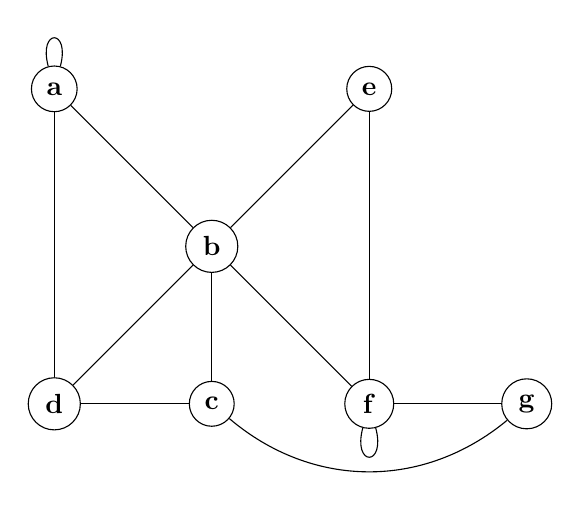
\begin{tikzpicture}[every loop/.style={}]
	\node[shape=circle,draw=black] (a) at (0, 4)     {\textbf{a}};
	\node[shape=circle,draw=black] (b) at (2, 2)     {\textbf{b}};
	\node[shape=circle,draw=black] (c) at (2, 0)     {\textbf{c}};
	\node[shape=circle,draw=black] (d) at (0, 0)     {\textbf{d}};
	\node[shape=circle,draw=black] (e) at (4, 4)     {\textbf{e}};
	\node[shape=circle,draw=black] (f) at (4, 0)     {\textbf{f}};
	\node[shape=circle,draw=black] (g) at (6, 0)     {\textbf{g}};
    \path[-] (a) edge (b);
    \path[-] (b) edge (d);
    \path[-] (d) edge (c);
    \path[-] (e) edge (b);
    \path[-] (f) edge (b);
    \path[-] (g) edge (f);
    \path[-] (a) edge (d);
    \path[-] (c) edge (b);
    \path[-] (e) edge (f);
    \path[-] (g) edge [bend left=40] (c);
    \path[every node/.style={font=\sffamily\small}]
        (a)   edge[loop above] (a);
    \path[every node/.style={font=\sffamily\small}]
        (f)   edge[loop below] (f);
	\end{tikzpicture} 
	\caption{The Underlying Undirected Graph of Graph G in Q2.}	
	\label{g2}
\end{figure}
    \item Since all vertices are connected to at least one other vertex, we can create paths between any given two vertices. % (Since the sub-graphs $(a, b, d)$, $(e,b,f)$, $(d,c,b)$, and $(b,c,g,f)$ are all complete loops).
    \item By using the Definition 5 from the Section 10.4 of the book, 
    \begin{quote}
        A directed graph is \textit{weakly connected} if there is a path between every two vertices in the underlying undirected graph.
    \end{quote}
    we can say that \textit{Graph G} is \textbf{weakly-connected}.
\end{itemize}

\subsection*{g}
The strongly-connected components of $G$ are as follows;
\begin{itemize}
    \item the vertex $a$
    \item the vertex $d$
    \item the vertex $g$
    \item the subgraph consisting of the vertices $b,c$ and edges $(b,c)$
    \item the subgraph consisting of the vertices $e,f$ and edges $(e,f)$
\end{itemize}
\subsection*{h}
By using the adjacency matrix from \textbf{part b}, we can generate the following adjacency matrix for the subgraph $H$ of $G$. 

\begin{figure}[H]
$$ A=  \begin{bmatrix}
        1 & 1 & 0 & 1 \\
        0 & 0 & 1 & 1 \\
        0 & 1 & 0 & 0 \\
        0 & 0 & 1 & 0 \\
    \end{bmatrix} $$
    \caption{Adjacency Matrix for Subgraph H}
\end{figure}

Since we need to find the number of different paths of length $3$, we need the $A^3$ matrix. (By using the Theorem 2 from the Section 10.4 of the book)

\begin{figure}[H]
$$ A^3=  \begin{bmatrix}
        1 & 3 & 3 & 2 \\
        0 & 1 & 1 & 1 \\
        0 & 1 & 1 & 0 \\
        0 & 0 & 1 & 1 \\
    \end{bmatrix} $$
\end{figure}
Therefore there are;
\begin{itemize}
    \item \textbf{1} path on $a \rightarrow a$
    \item \textbf{3} paths on $a \rightarrow b$
    \item \textbf{3} paths on $a \rightarrow c$
    \item \textbf{2} paths on $a \rightarrow d$
    \item \textbf{0} paths on $b \rightarrow a$
    \item \textbf{1} path on $b \rightarrow b$
    \item \textbf{1} path on $b \rightarrow c$
    \item \textbf{1} path on $b \rightarrow d$
    \item \textbf{0} paths on $c \rightarrow a$
    \item \textbf{1} path on $c \rightarrow b$
    \item \textbf{1} paths on $c \rightarrow c$
    \item \textbf{0} paths on $c \rightarrow d$
    \item \textbf{0} paths on $d \rightarrow a$
    \item \textbf{0} paths on $d \rightarrow b$
    \item \textbf{1} path on $d \rightarrow c$
    \item \textbf{1} path on $d \rightarrow d$
\end{itemize}
exist.

\section*{Answer 3}
\begin{table}[H]
    \centering
    \renewcommand{\arraystretch}{1.25}
    \begin{tabular}{|l||c|c|c|c|c|c|c|c|c|c|c|}	
    \hline 							
    \textbf{Vertex} & a & b & c & d & e & f & g & h & i & j & k  \\ \hline
    \textbf{Degree} & 2 & 6 & 4 & 4 & 6 & 6 & 4 & 4 & 4 & 6 & 2 \\ \hline
    \end{tabular}
    \caption{ Degrees of each Vertex in Graph G in Q3 }
    \label{tq3}
    \end{table}

\subsection*{a}
\begin{itemize}
    \item  \textbf{Theorem 2} from the Section 10.5 of the textbook says that 
    \begin{quote}
        A connected multigraph has an Euler path but not an Euler circuit if and only if it has exactly two vertices of odd degree.
    \end{quote}
    \item Since the \textit{Graph G} is a connected multigraph, to check if the given graph has an Euler Path, we can simply check the degree of each vertex. On a graph with $n$ vertices, if $n-2$ vertices have even degree, and if the remaining 2 vertices have odd degrees, the given graph has an \textbf{Euler Path}. 
    \item When we look at Table \ref{tq3}, we can clearly see that all vertices are of even degree. 
    \item Therefore, \textit{Graph G} does not have an \textbf{Euler Path}. 
\end{itemize}

\subsection*{b}
\begin{itemize}
    \item  \textbf{Theorem 1} from the Section 10.5 of the textbook says that 
    \begin{quote}
        A connected multigraph with at least two vertices has an Euler circuit if and only if each of its vertices has even degree.
    \end{quote}
    \item Since the \textit{Graph G} is a connected multigraph with 11 vertices, to check if the given graph has an Euler Path, we can simply check the degree of each vertex. If all vertices have even degree, the given graph has an \textbf{Euler Circuit}. 
    \item When we look at Table \ref{tq3}, we can clearly see that all vertices are of even degree. 
    \item Therefore, \textit{Graph G} has an \textbf{Euler Circuit}. 
    \item An example \textbf{Euler Circuit}: $ j \rightarrow j \rightarrow c \rightarrow f \rightarrow e \rightarrow a \rightarrow b \rightarrow b \rightarrow e \rightarrow f \rightarrow b \rightarrow f \rightarrow i \rightarrow e \rightarrow h \rightarrow h \rightarrow i \rightarrow c \rightarrow d \rightarrow g \rightarrow j \rightarrow k \rightarrow g \rightarrow d$
\end{itemize}

\subsection*{c}

\begin{itemize}
    \item  \textbf{Definition 2} from the Section 10.5 of the textbook says that 
    \begin{quote}
        A simple path in a \textit{Graph G} that passes through every vertex exactly once is called a \textit{Hamilton Path}.
    \end{quote}
    
    \item By picking the following simple route, we can create a \textit{Hamilton Path};
    \subitem $ k \rightarrow j \rightarrow g \rightarrow d \rightarrow c \rightarrow i \rightarrow h \rightarrow e \rightarrow a \rightarrow b \rightarrow f $
    \item Since we  were able to create a \textit{Hamilton Path}, we can say that \textit{Graph G} has a \textbf{Hamilton Path}. 
\end{itemize}

\subsection*{d}
\begin{itemize}
    \item  \textbf{Theorem 4 (Ore's Theorem)} from the Section 10.5 of the textbook says that 
    \begin{quote}
        If $G$ is a simple graph with $n$ vertices with $n \geq 3$ such that
$deg(u) + deg(v) \geq n$ for every pair of nonadjacent vertices $u$ and $v$ in $G$, then $G$ has a \textit{Hamilton Circuit}.
    \end{quote}
    \item Since the \textit{Graph G} is a simple graph with 11 vertices, if we find a pair of nonadjacent vertices with summed degrees less than 11, we can say that the given graph does not have a \textbf{Hamilton Circuit}. 
    \item Let us pick the nonadjacent vertices $a$ and $k$. When we look at Table \ref{tq3}, we can see that their degrees are 2 and 2, respectively. 
    \item We can easily see that $deg(a) + deg(k) \geq 11$ does not hold, and therefore  \textit{Graph G} does not have a \textbf{Hamilton Circuit}. 
\end{itemize}

\section*{Answer 4}
\subsection*{a}
\begin{itemize}
    \item By the definition of the \textit{Complete Bipartite Graph}, $K_{m,n}$ has two different subsets of vertices, namely $m$ and $n$ vertices each.
    \item Therefore, the total number of vertices are $m+n$.
    \item Since each vertex from the subset $m$ will have edges with each vertex from subset $n$, we can say that the total number of edges are $m \cdot n$.
\end{itemize}
\subsection*{b}
\begin{itemize}
    \item  \textbf{Theorem 4 (Ore's Theorem)} from the Section 10.5 of the textbook says that 
    \begin{quote}
        If $G$ is a simple graph with $n$ vertices with $n \geq 3$ such that
$deg(u) + deg(v) \geq n$ for every pair of nonadjacent vertices $u$ and $v$ in $G$, then $G$ has a \textit{Hamilton Circuit}.
    \end{quote}
    \item Since \textit{Complete Bipartite Graphs} are simple, we can continue with the further requirements.
    \item Let us say $m + n = \beta$, and since m is odd and n is even, $\beta > 3$ also holds. 
    \item Since each vertex in subset m has edges with each vertex in subset n, the only nonadjacent vertices are the vertices within the same subset. 
    \item Each vertex in subset m will have exactly n edges; similarly each vertex in subset n will have exactly m edges.
    \item By applying \textit{Ore's Theorem} to two vertices in subset m, we get; 
    \begin{center} $ deg(m_i) + deg(m_j) \geq m+n $, where $m_i, m_j \in m$ \end{center}
    \item Since the degree of each vertex in $m$ is $n$, we can write the following;
    \begin{center} $ n + n \geq m + n $ \end{center}
    \begin{equation} n \geq m  
    \label{q421}
    \end{equation} 
    \item Similarly, by applying \textit{Ore's Theorem} to two vertices in subset n, we get;
    \begin{center} $ deg(n_p) + deg(n_r) \geq m+n $, where $n_p, n_r \in n$ \end{center}
    \item Since the degree of each vertex in $n$ is $m$, we can write the following;
    \begin{center} $ m + m \geq m + n $ \end{center}
    \begin{equation} m \geq n 
    \label{q422} \end{equation} 
    \item By combining inequalities \eqref{q421} and \eqref{q422}, we can see that the solution only exists when $m = n$. Since by the initial conditions we are given that $m$ is odd and $n$ is even, $m=n$ does not hold. Therefore, we can conclude that $K_{m,n}$ with odd $m$ and even $n$ does not have a Hamiltonian circuit.
\end{itemize} 

\section*{Answer 5}
\subsection*{a}
\subsubsection*{Step 0}
For this question, I used superscripts in the nodes as shortest distances from the starting node, namely $s$, for this graph.
\begin{figure}[H]
	\centering
	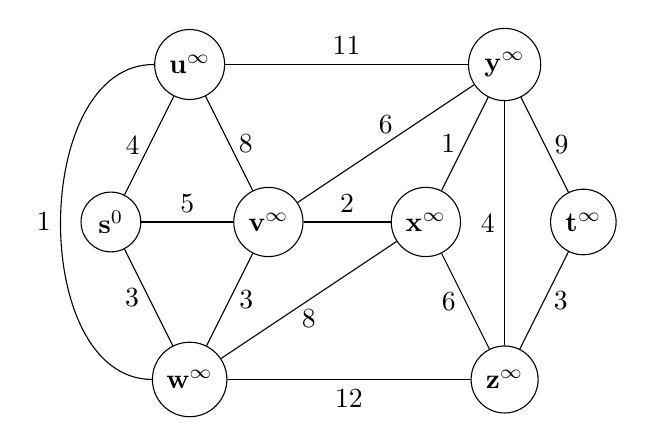
\begin{tikzpicture}
	\node[shape=circle,draw=black] (s) at (1, 2)     {\textbf{s$^0$}};
	\node[shape=circle,draw=black] (u) at (2, 4)     {\textbf{u$^\infty$}};
	\node[shape=circle,draw=black] (v) at (3, 2)     {\textbf{v$^\infty$}};
	\node[shape=circle,draw=black] (w) at (2, 0)     {\textbf{w$^\infty$}};
	\node[shape=circle,draw=black] (x) at (5, 2)     {\textbf{x$^\infty$}};
	\node[shape=circle,draw=black] (y) at (6, 4)     {\textbf{y$^\infty$}};
	\node[shape=circle,draw=black] (z) at (6, 0)     {\textbf{z$^\infty$}};
	\node[shape=circle,draw=black] (t) at (7, 2)     {\textbf{t$^\infty$}};
	\path[-] (s) edge node[left]{4} (u);
	\path[-] (s) edge node[above]{5} (v);
	\path[-] (u) edge [bend right=90] node[left]{1} (w);
	\path[-] (u) edge node[above]{11} (y);
	\path[-] (u) edge node[right]{8} (v);
	\path[-] (v) edge node[above]{6} (y);
	\path[-] (v) edge node[above]{2} (x);
	\path[-] (v) edge node[right]{3} (w);
	\path[-] (w) edge node[left]{3} (s);
	\path[-] (w) edge node[below]{8} (x);
	\path[-] (w) edge node[below]{12} (z);
	\path[-] (x) edge node[left]{1} (y);
	\path[-] (x) edge node[left]{6} (z);
	\path[-] (y) edge node[left]{4} (z);
	\path[-] (y) edge node[right]{9} (t);
	\path[-] (z) edge node[right]{3} (t);
	\end{tikzpicture} 
	\caption{Initial condition}
\end{figure}

\subsubsection*{Step 1}
By visiting the \textit{unvisited} neighbouring nodes of $s$, we get the following graph.
\begin{figure}[H]
	\centering
	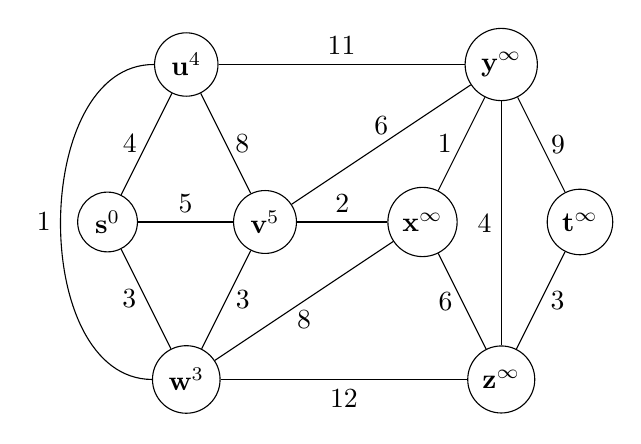
\begin{tikzpicture}
	\node[shape=circle,draw=black] (s) at (1, 2)     {\textbf{s$^0$}};
	\node[shape=circle,draw=black] (u) at (2, 4)     {\textbf{u$^4$}};
	\node[shape=circle,draw=black] (v) at (3, 2)     {\textbf{v$^5$}};
	\node[shape=circle,draw=black] (w) at (2, 0)     {\textbf{w$^3$}};
	\node[shape=circle,draw=black] (x) at (5, 2)     {\textbf{x$^\infty$}};
	\node[shape=circle,draw=black] (y) at (6, 4)     {\textbf{y$^\infty$}};
	\node[shape=circle,draw=black] (z) at (6, 0)     {\textbf{z$^\infty$}};
	\node[shape=circle,draw=black] (t) at (7, 2)     {\textbf{t$^\infty$}};
	\path[-] (s) edge node[left]{4} (u);
	\path[-] (s) edge node[above]{5} (v);
	\path[-] (u) edge [bend right=90] node[left]{1} (w);
	\path[-] (u) edge node[above]{11} (y);
	\path[-] (u) edge node[right]{8} (v);
	\path[-] (v) edge node[above]{6} (y);
	\path[-] (v) edge node[above]{2} (x);
	\path[-] (v) edge node[right]{3} (w);
	\path[-] (w) edge node[left]{3} (s);
	\path[-] (w) edge node[below]{8} (x);
	\path[-] (w) edge node[below]{12} (z);
	\path[-] (x) edge node[left]{1} (y);
	\path[-] (x) edge node[left]{6} (z);
	\path[-] (y) edge node[left]{4} (z);
	\path[-] (y) edge node[right]{9} (t);
	\path[-] (z) edge node[right]{3} (t);
	\end{tikzpicture} 
	\caption{The graph after node $s$ has visited}
\end{figure}
The distance costs and routes from node $s$ are as follows;
\begin{itemize}
    \item w: 3 (s)
    \item u: 4 (s)
    \item v: 5 (s)
\end{itemize}
\textbf{Visited Nodes} : s

\subsubsection*{Step 2}
By visiting the \textit{unvisited} neighbouring nodes of $w$, we get the following graph.
\begin{figure}[H]
	\centering
	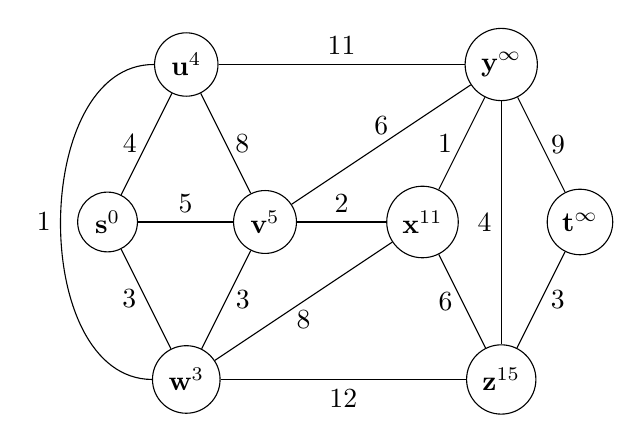
\begin{tikzpicture}
	\node[shape=circle,draw=black] (s) at (1, 2)     {\textbf{s$^0$}};
	\node[shape=circle,draw=black] (u) at (2, 4)     {\textbf{u$^4$}};
	\node[shape=circle,draw=black] (v) at (3, 2)     {\textbf{v$^5$}};
	\node[shape=circle,draw=black] (w) at (2, 0)     {\textbf{w$^3$}};
	\node[shape=circle,draw=black] (x) at (5, 2)     {\textbf{x$^{11}$}};
	\node[shape=circle,draw=black] (y) at (6, 4)     {\textbf{y$^\infty$}};
	\node[shape=circle,draw=black] (z) at (6, 0)     {\textbf{z$^{15}$}};
	\node[shape=circle,draw=black] (t) at (7, 2)     {\textbf{t$^\infty$}};
	\path[-] (s) edge node[left]{4} (u);
	\path[-] (s) edge node[above]{5} (v);
	\path[-] (u) edge [bend right=90] node[left]{1} (w);
	\path[-] (u) edge node[above]{11} (y);
	\path[-] (u) edge node[right]{8} (v);
	\path[-] (v) edge node[above]{6} (y);
	\path[-] (v) edge node[above]{2} (x);
	\path[-] (v) edge node[right]{3} (w);
	\path[-] (w) edge node[left]{3} (s);
	\path[-] (w) edge node[below]{8} (x);
	\path[-] (w) edge node[below]{12} (z);
	\path[-] (x) edge node[left]{1} (y);
	\path[-] (x) edge node[left]{6} (z);
	\path[-] (y) edge node[left]{4} (z);
	\path[-] (y) edge node[right]{9} (t);
	\path[-] (z) edge node[right]{3} (t);
	\end{tikzpicture} 
	\caption{The graph after node $w$ has visited}
\end{figure}
The distance costs and routes from node $s$ are as follows;
\begin{itemize}
    \item w: 3 (s)
    \item u: 4 (s)
    \item v: 5 (s)
    \item x: 11 (s,w)
    \item z: 15 (s,w)
\end{itemize}
\textbf{Visited Nodes} : s, w

\subsubsection*{Step 3}
By visiting the \textit{unvisited} neighbouring nodes of $u$, we get the following graph.
\begin{figure}[H]
	\centering
	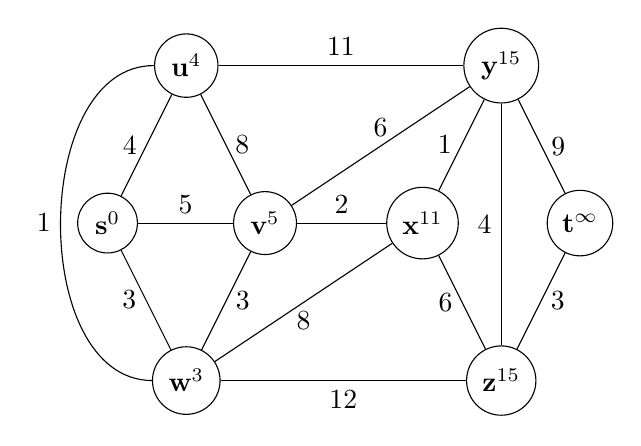
\begin{tikzpicture}
	\node[shape=circle,draw=black] (s) at (1, 2)     {\textbf{s$^0$}};
	\node[shape=circle,draw=black] (u) at (2, 4)     {\textbf{u$^4$}};
	\node[shape=circle,draw=black] (v) at (3, 2)     {\textbf{v$^5$}};
	\node[shape=circle,draw=black] (w) at (2, 0)     {\textbf{w$^3$}};
	\node[shape=circle,draw=black] (x) at (5, 2)     {\textbf{x$^{11}$}};
	\node[shape=circle,draw=black] (y) at (6, 4)     {\textbf{y$^{15}$}};
	\node[shape=circle,draw=black] (z) at (6, 0)     {\textbf{z$^{15}$}};
	\node[shape=circle,draw=black] (t) at (7, 2)     {\textbf{t$^\infty$}};
	\path[-] (s) edge node[left]{4} (u);
	\path[-] (s) edge node[above]{5} (v);
	\path[-] (u) edge [bend right=90] node[left]{1} (w);
	\path[-] (u) edge node[above]{11} (y);
	\path[-] (u) edge node[right]{8} (v);
	\path[-] (v) edge node[above]{6} (y);
	\path[-] (v) edge node[above]{2} (x);
	\path[-] (v) edge node[right]{3} (w);
	\path[-] (w) edge node[left]{3} (s);
	\path[-] (w) edge node[below]{8} (x);
	\path[-] (w) edge node[below]{12} (z);
	\path[-] (x) edge node[left]{1} (y);
	\path[-] (x) edge node[left]{6} (z);
	\path[-] (y) edge node[left]{4} (z);
	\path[-] (y) edge node[right]{9} (t);
	\path[-] (z) edge node[right]{3} (t);
	\end{tikzpicture} 
	\caption{The graph after node $u$ has visited}
\end{figure}
The distance costs and routes from node $s$ are as follows;
\begin{itemize}
    \item w: 3 (s)
    \item u: 4 (s)
    \item v: 5 (s)
    \item x: 11 (s,w)
    \item z: 15 (s,w)
    \item y: 15 (s,u)
\end{itemize}
\textbf{Visited Nodes} : s, w, u

\subsubsection*{Step 4}
By visiting the \textit{unvisited} neighbouring nodes of $v$, we get the following graph.
\begin{figure}[H]
	\centering
	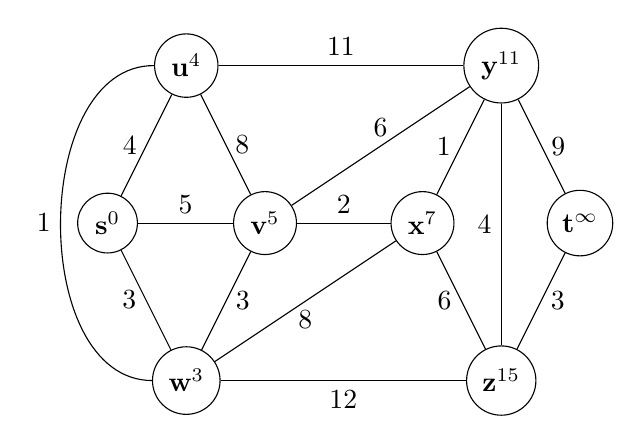
\begin{tikzpicture}
	\node[shape=circle,draw=black] (s) at (1, 2)     {\textbf{s$^0$}};
	\node[shape=circle,draw=black] (u) at (2, 4)     {\textbf{u$^4$}};
	\node[shape=circle,draw=black] (v) at (3, 2)     {\textbf{v$^5$}};
	\node[shape=circle,draw=black] (w) at (2, 0)     {\textbf{w$^3$}};
	\node[shape=circle,draw=black] (x) at (5, 2)     {\textbf{x$^{7}$}};
	\node[shape=circle,draw=black] (y) at (6, 4)     {\textbf{y$^{11}$}};
	\node[shape=circle,draw=black] (z) at (6, 0)     {\textbf{z$^{15}$}};
	\node[shape=circle,draw=black] (t) at (7, 2)     {\textbf{t$^\infty$}};
	\path[-] (s) edge node[left]{4} (u);
	\path[-] (s) edge node[above]{5} (v);
	\path[-] (u) edge [bend right=90] node[left]{1} (w);
	\path[-] (u) edge node[above]{11} (y);
	\path[-] (u) edge node[right]{8} (v);
	\path[-] (v) edge node[above]{6} (y);
	\path[-] (v) edge node[above]{2} (x);
	\path[-] (v) edge node[right]{3} (w);
	\path[-] (w) edge node[left]{3} (s);
	\path[-] (w) edge node[below]{8} (x);
	\path[-] (w) edge node[below]{12} (z);
	\path[-] (x) edge node[left]{1} (y);
	\path[-] (x) edge node[left]{6} (z);
	\path[-] (y) edge node[left]{4} (z);
	\path[-] (y) edge node[right]{9} (t);
	\path[-] (z) edge node[right]{3} (t);
	\end{tikzpicture} 
	\caption{The graph after node $v$ has visited}
\end{figure}
The distance costs and routes from node $s$ are as follows;
\begin{itemize}
    \item w: 3 (s)
    \item u: 4 (s)
    \item v: 5 (s)
    \item x: 7 (s,v)
    \item y: 11 (s,v)
    \item z: 15 (s,w)
\end{itemize}
\textbf{Visited Nodes} : s, w, u, v

\subsubsection*{Step 5}
By visiting the \textit{unvisited} neighbouring nodes of $x$, we get the following graph.
\begin{figure}[H]
	\centering
	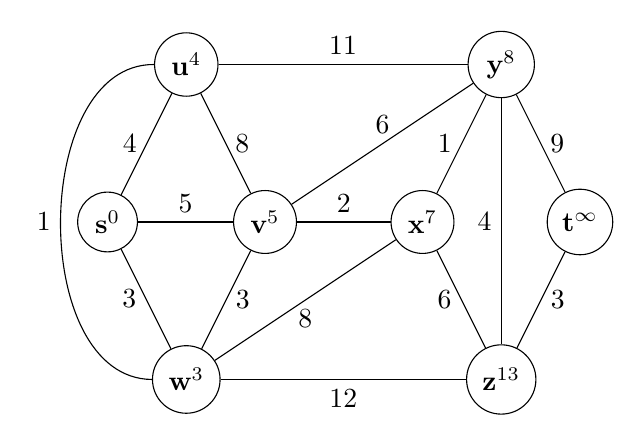
\begin{tikzpicture}
	\node[shape=circle,draw=black] (s) at (1, 2)     {\textbf{s$^0$}};
	\node[shape=circle,draw=black] (u) at (2, 4)     {\textbf{u$^4$}};
	\node[shape=circle,draw=black] (v) at (3, 2)     {\textbf{v$^5$}};
	\node[shape=circle,draw=black] (w) at (2, 0)     {\textbf{w$^3$}};
	\node[shape=circle,draw=black] (x) at (5, 2)     {\textbf{x$^{7}$}};
	\node[shape=circle,draw=black] (y) at (6, 4)     {\textbf{y$^{8}$}};
	\node[shape=circle,draw=black] (z) at (6, 0)     {\textbf{z$^{13}$}};
	\node[shape=circle,draw=black] (t) at (7, 2)     {\textbf{t$^\infty$}};
	\path[-] (s) edge node[left]{4} (u);
	\path[-] (s) edge node[above]{5} (v);
	\path[-] (u) edge [bend right=90] node[left]{1} (w);
	\path[-] (u) edge node[above]{11} (y);
	\path[-] (u) edge node[right]{8} (v);
	\path[-] (v) edge node[above]{6} (y);
	\path[-] (v) edge node[above]{2} (x);
	\path[-] (v) edge node[right]{3} (w);
	\path[-] (w) edge node[left]{3} (s);
	\path[-] (w) edge node[below]{8} (x);
	\path[-] (w) edge node[below]{12} (z);
	\path[-] (x) edge node[left]{1} (y);
	\path[-] (x) edge node[left]{6} (z);
	\path[-] (y) edge node[left]{4} (z);
	\path[-] (y) edge node[right]{9} (t);
	\path[-] (z) edge node[right]{3} (t);
	\end{tikzpicture} 
	\caption{The graph after node $x$ has visited}
\end{figure}
The distance costs and routes from node $s$ are as follows;
\begin{itemize}
    \item w: 3 (s)
    \item u: 4 (s)
    \item v: 5 (s)
    \item x: 7 (s,v)
    \item y: 8 (s,v,x)
    \item z: 13 (s,v,x)
\end{itemize}
\textbf{Visited Nodes} : s, w, u, v, x

\subsubsection*{Step 6}
By visiting the \textit{unvisited} neighbouring nodes of $y$, we get the following graph.
\begin{figure}[H]
	\centering
	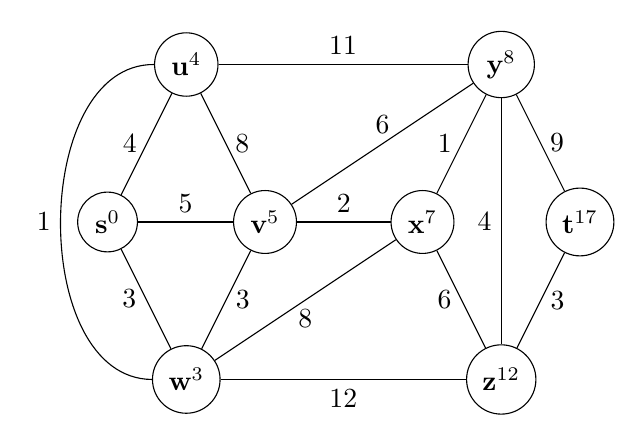
\begin{tikzpicture}
	\node[shape=circle,draw=black] (s) at (1, 2)     {\textbf{s$^0$}};
	\node[shape=circle,draw=black] (u) at (2, 4)     {\textbf{u$^4$}};
	\node[shape=circle,draw=black] (v) at (3, 2)     {\textbf{v$^5$}};
	\node[shape=circle,draw=black] (w) at (2, 0)     {\textbf{w$^3$}};
	\node[shape=circle,draw=black] (x) at (5, 2)     {\textbf{x$^{7}$}};
	\node[shape=circle,draw=black] (y) at (6, 4)     {\textbf{y$^{8}$}};
	\node[shape=circle,draw=black] (z) at (6, 0)     {\textbf{z$^{12}$}};
	\node[shape=circle,draw=black] (t) at (7, 2)     {\textbf{t$^{17}$}};
	\path[-] (s) edge node[left]{4} (u);
	\path[-] (s) edge node[above]{5} (v);
	\path[-] (u) edge [bend right=90] node[left]{1} (w);
	\path[-] (u) edge node[above]{11} (y);
	\path[-] (u) edge node[right]{8} (v);
	\path[-] (v) edge node[above]{6} (y);
	\path[-] (v) edge node[above]{2} (x);
	\path[-] (v) edge node[right]{3} (w);
	\path[-] (w) edge node[left]{3} (s);
	\path[-] (w) edge node[below]{8} (x);
	\path[-] (w) edge node[below]{12} (z);
	\path[-] (x) edge node[left]{1} (y);
	\path[-] (x) edge node[left]{6} (z);
	\path[-] (y) edge node[left]{4} (z);
	\path[-] (y) edge node[right]{9} (t);
	\path[-] (z) edge node[right]{3} (t);
	\end{tikzpicture} 
	\caption{The graph after node $y$ has visited}
\end{figure}
The distance costs and routes from node $s$ are as follows;
\begin{itemize}
    \item w: 3 (s)
    \item u: 4 (s)
    \item v: 5 (s)
    \item x: 7 (s,v)
    \item y: 8 (s,v,x)
    \item z: 12 (s,v,x,y)
    \item t: 17 (s,v,x,y)
\end{itemize}
\textbf{Visited Nodes} : s, w, u, v, x, y


\subsubsection*{Step 7}
By visiting the \textit{unvisited} neighbouring nodes of $z$, we get the following graph.
\begin{figure}[H]
	\centering
	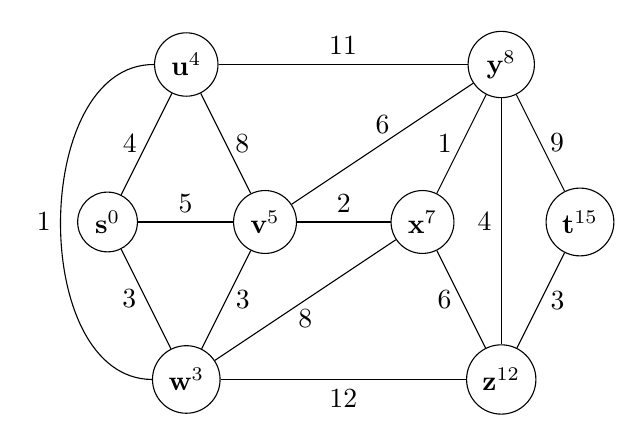
\begin{tikzpicture}
	\node[shape=circle,draw=black] (s) at (1, 2)     {\textbf{s$^0$}};
	\node[shape=circle,draw=black] (u) at (2, 4)     {\textbf{u$^4$}};
	\node[shape=circle,draw=black] (v) at (3, 2)     {\textbf{v$^5$}};
	\node[shape=circle,draw=black] (w) at (2, 0)     {\textbf{w$^3$}};
	\node[shape=circle,draw=black] (x) at (5, 2)     {\textbf{x$^{7}$}};
	\node[shape=circle,draw=black] (y) at (6, 4)     {\textbf{y$^{8}$}};
	\node[shape=circle,draw=black] (z) at (6, 0)     {\textbf{z$^{12}$}};
	\node[shape=circle,draw=black] (t) at (7, 2)     {\textbf{t$^{15}$}};
	\path[-] (s) edge node[left]{4} (u);
	\path[-] (s) edge node[above]{5} (v);
	\path[-] (u) edge [bend right=90] node[left]{1} (w);
	\path[-] (u) edge node[above]{11} (y);
	\path[-] (u) edge node[right]{8} (v);
	\path[-] (v) edge node[above]{6} (y);
	\path[-] (v) edge node[above]{2} (x);
	\path[-] (v) edge node[right]{3} (w);
	\path[-] (w) edge node[left]{3} (s);
	\path[-] (w) edge node[below]{8} (x);
	\path[-] (w) edge node[below]{12} (z);
	\path[-] (x) edge node[left]{1} (y);
	\path[-] (x) edge node[left]{6} (z);
	\path[-] (y) edge node[left]{4} (z);
	\path[-] (y) edge node[right]{9} (t);
	\path[-] (z) edge node[right]{3} (t);
	\end{tikzpicture} 
	\caption{The graph after node $y$ has visited}
\end{figure}
The distance costs and routes from node $s$ are as follows;
\begin{itemize}
    \item w: 3 (s)
    \item u: 4 (s)
    \item v: 5 (s)
    \item x: 7 (s,v)
    \item y: 8 (s,v,x)
    \item z: 12 (s,v,x,y)
    \item t: 15 (s,v,x,y,z)
\end{itemize}
\textbf{Visited Nodes} : s, w, u, v, x, y, z

\subsubsection*{Step 8}
Since there are no \textit{unvisited} neighbouring nodes of $t$, we concluded our traversal. \\
The shortest path from $s$ to $t$ by using \textbf{Dijkstra's Algorithm} is: $ s \rightarrow v \rightarrow x \rightarrow y \rightarrow z \rightarrow t$, and it has a distance cost of $15$.

\subsection*{b}
By following the choices below, 
\begin{table}[H]
    \centering
    \renewcommand{\arraystretch}{1.25}
    \begin{tabular}{|c|c|c|p{114mm}|}	
    \hline 							
   \textbf{Choice} & \textbf{Edge} & \textbf{Weight} & \textbf{Reason} \\
    \hline 
    \hline 
    1 & [x,y] & 1 & From the vertex $x$, we start with picking the smallest weighted edge. \\ \hline
    2 & [x,v] & 2 & From the vertices $x$ and $y$, the smallest weighted edge is $x-v$, with a weight of 2. \\ \hline
    3 & [v,w] & 3 & From the vertices $x$, $y$ and $v$, the smallest weighted edge is $v-w$, with a weight of 3.\\ \hline
    4 & [w,u] & 1 & From the vertices $x$, $y$, $v$ and $w$, the smallest weighted edge is $w-u$, with a weight of 1.\\ \hline
    5 & [w,s] & 3 & From the vertices $x$, $y$, $v$, $w$ and $u$, the smallest weighted edge is $w-s$, with a weight of 3. \\ \hline
    6 & [y,z] & 4 & From the vertices $x$, $y$, $v$, $w$, $u$ and $s$, the smallest weighted edges are $s-u$ and $y-z$, with weights of 4. But since picking $u-s$ would form a \textit{simple circuit}, we cannot pick it. Therefore we pick $y-z$. \\ \hline
    7 & [z,t] & 3 & From the vertices $x$, $y$, $v$, $w$, $u$, $s$ and $z$, the smallest weighted edge is $z-t$, with a weight of 3. \\ \hline
    \end{tabular}
    \caption{ Procedure of creating a minimum spanning tree of Graph G in Q5 produced using Prim's Algorithm }
    \end{table}
    
we conclude the minimum spanning tree, since picking any of the remaining edges would form \textit{simple circuits}. 

The minimum spanning tree of the graph can be seen above (the used edges are denoted with a \textit{ultra thick} edge).

\begin{figure}[H]
	\centering
	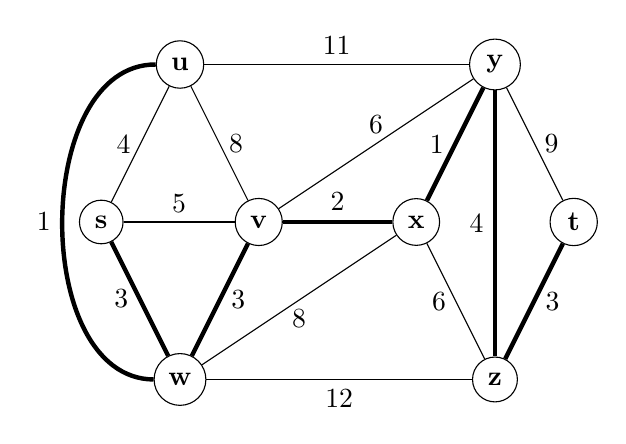
\begin{tikzpicture}
	\node[shape=circle,draw=black] (s) at (1, 2)     {\textbf{s}};
	\node[shape=circle,draw=black] (u) at (2, 4)     {\textbf{u}};
	\node[shape=circle,draw=black] (v) at (3, 2)     {\textbf{v}};
	\node[shape=circle,draw=black] (w) at (2, 0)     {\textbf{w}};
	\node[shape=circle,draw=black] (x) at (5, 2)     {\textbf{x}};
	\node[shape=circle,draw=black] (y) at (6, 4)     {\textbf{y}};
	\node[shape=circle,draw=black] (z) at (6, 0)     {\textbf{z}};
	\node[shape=circle,draw=black] (t) at (7, 2)     {\textbf{t}};

	\path[-] (s) edge node[left]{4} (u);
	\path[-] (s) edge node[above]{5} (v);
	\path[ultra thick] (u) edge [bend right=90] node[left]{1} (w);
	\path[-] (u) edge node[above]{11} (y);
	\path[-] (u) edge node[right]{8} (v);
	\path[-] (v) edge node[above]{6} (y);
	\path[ultra thick] (v) edge node[above]{2} (x);
	\path[ultra thick] (v) edge node[right]{3} (w);
	\path[ultra thick] (w) edge node[left]{3} (s);
	\path[-] (w) edge node[below]{8} (x);
	\path[-] (w) edge node[below]{12} (z);
	\path[ultra thick] (x) edge node[left]{1} (y);
	\path[-] (x) edge node[left]{6} (z);
	\path[ultra thick] (y) edge node[left]{4} (z);
	\path[-] (y) edge node[right]{9} (t);
	\path[ultra thick] (z) edge node[right]{3} (t);
		
	\end{tikzpicture} 
	\caption{A minimum spanning tree of Graph G in Q5 produced using Prim's Algorithm}
	\label{g5}
\end{figure}

\subsection*{c}

The initial minimum spanning tree of the graph as follows (the used edges are denoted with a \textit{ultra thick} edge).

\begin{figure}[H]
	\centering
	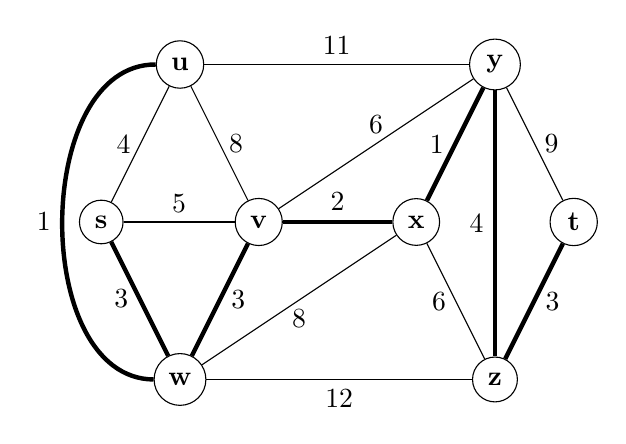
\begin{tikzpicture}
	\node[shape=circle,draw=black] (s) at (1, 2)     {\textbf{s}};
	\node[shape=circle,draw=black] (u) at (2, 4)     {\textbf{u}};
	\node[shape=circle,draw=black] (v) at (3, 2)     {\textbf{v}};
	\node[shape=circle,draw=black] (w) at (2, 0)     {\textbf{w}};
	\node[shape=circle,draw=black] (x) at (5, 2)     {\textbf{x}};
	\node[shape=circle,draw=black] (y) at (6, 4)     {\textbf{y}};
	\node[shape=circle,draw=black] (z) at (6, 0)     {\textbf{z}};
	\node[shape=circle,draw=black] (t) at (7, 2)     {\textbf{t}};

	\path[-] (s) edge node[left]{4} (u);
	\path[-] (s) edge node[above]{5} (v);
	\path[ultra thick] (u) edge [bend right=90] node[left]{1} (w);
	\path[-] (u) edge node[above]{11} (y);
	\path[-] (u) edge node[right]{8} (v);
	\path[-] (v) edge node[above]{6} (y);
	\path[ultra thick] (v) edge node[above]{2} (x);
	\path[ultra thick] (v) edge node[right]{3} (w);
	\path[ultra thick] (w) edge node[left]{3} (s);
	\path[-] (w) edge node[below]{8} (x);
	\path[-] (w) edge node[below]{12} (z);
	\path[ultra thick] (x) edge node[left]{1} (y);
	\path[-] (x) edge node[left]{6} (z);
	\path[ultra thick] (y) edge node[left]{4} (z);
	\path[-] (y) edge node[right]{9} (t);
	\path[ultra thick] (z) edge node[right]{3} (t);
		
	\end{tikzpicture} 
	\caption{A minimum spanning tree of Graph G in Q5 produced using Prim's Algorithm}
	\label{g6}
\end{figure}

\subsubsection*{Adding (s,x,1)}
\begin{figure}[H]
	\centering
	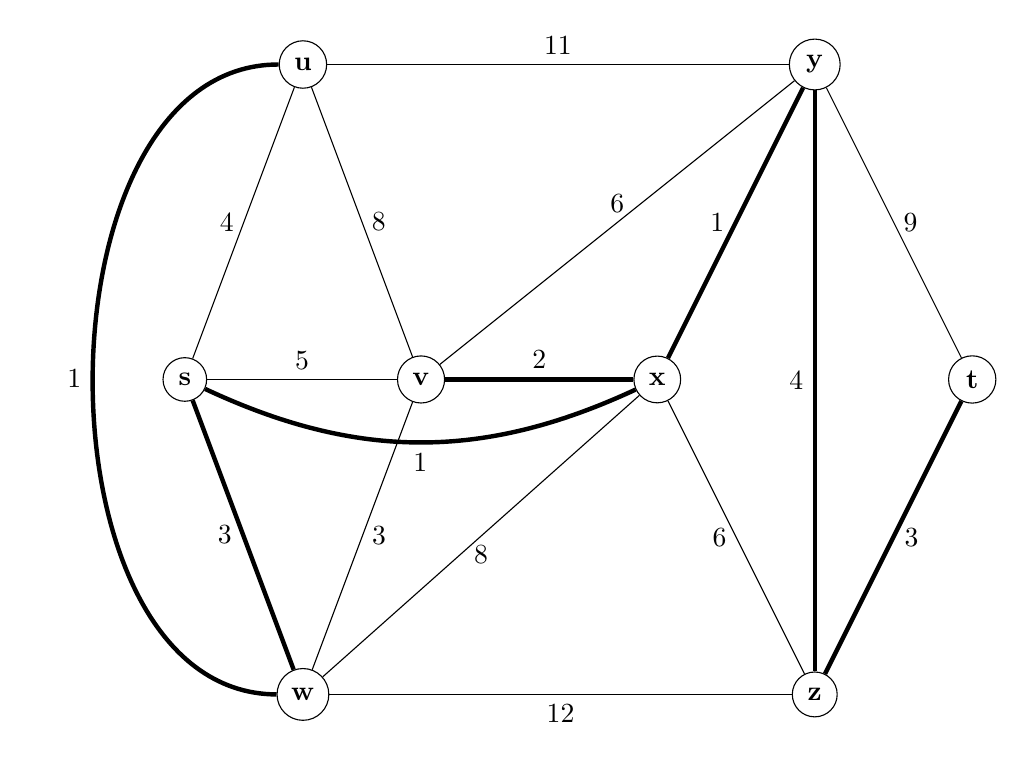
\begin{tikzpicture}
	\node[shape=circle,draw=black] (s) at (1, 4)     {\textbf{s}};
	\node[shape=circle,draw=black] (u) at (2.5, 8)     {\textbf{u}};
	\node[shape=circle,draw=black] (v) at (4, 4)     {\textbf{v}};
	\node[shape=circle,draw=black] (w) at (2.5, 0)     {\textbf{w}};
	\node[shape=circle,draw=black] (x) at (7, 4)     {\textbf{x}};
	\node[shape=circle,draw=black] (y) at (9, 8)     {\textbf{y}};
	\node[shape=circle,draw=black] (z) at (9, 0)     {\textbf{z}};
	\node[shape=circle,draw=black] (t) at (11, 4)     {\textbf{t}};

	\path[-] (s) edge node[left]{4} (u);
	\path[-] (s) edge node[above]{5} (v);
	\path[ultra thick] (u) edge [bend right=90] node[left]{1} (w);
	\path[-] (u) edge node[above]{11} (y);
	\path[-] (u) edge node[right]{8} (v);
	\path[ultra thick] (s) edge [bend right=25] node[below]{1} (x);
	\path[-] (v) edge node[above]{6} (y);
	\path[ultra thick] (v) edge node[above]{2} (x);
	\path[-] (v) edge node[right]{3} (w);
	\path[ultra thick] (w) edge node[left]{3} (s);
	\path[-] (w) edge node[below]{8} (x);
	\path[-] (w) edge node[below]{12} (z);
	\path[ultra thick] (x) edge node[left]{1} (y);
	\path[-] (x) edge node[left]{6} (z);
	\path[ultra thick] (y) edge node[left]{4} (z);
	\path[-] (y) edge node[right]{9} (t);
	\path[ultra thick] (z) edge node[right]{3} (t);
		
	\end{tikzpicture} 
	\caption{The minimum spanning tree of Graph G in Q5 after adding (s,x,1)}
	\label{g7}
\end{figure}

\subsubsection*{Adding (t,u,6)}
\begin{figure}[H]
	\centering
	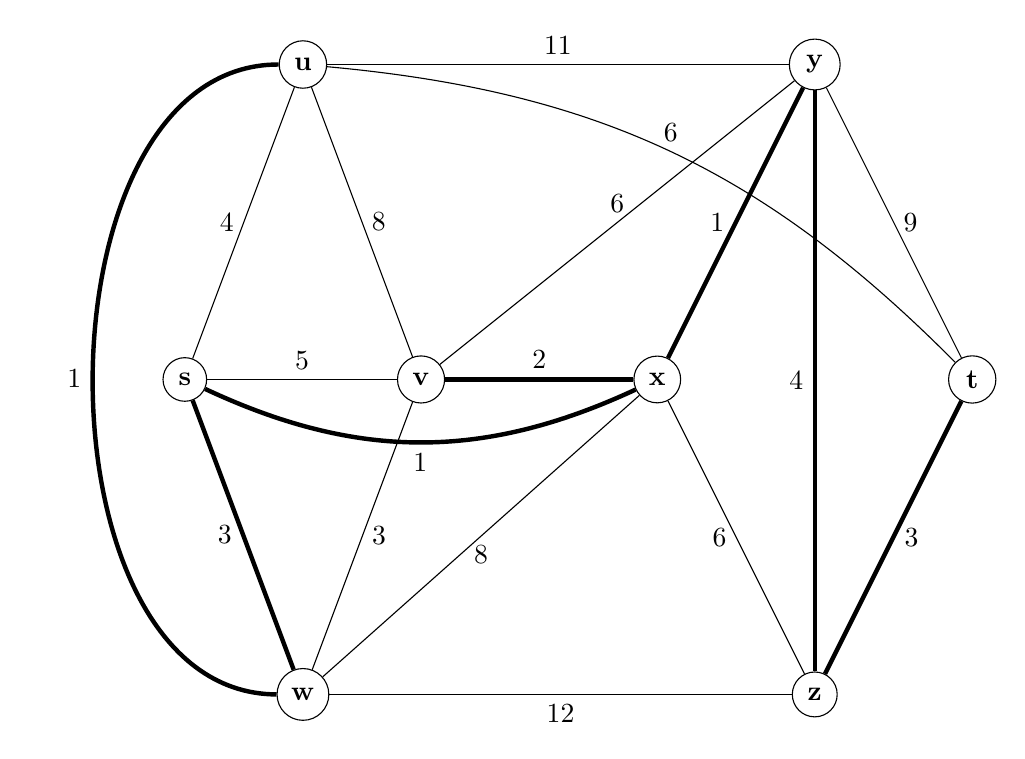
\begin{tikzpicture}
	\node[shape=circle,draw=black] (s) at (1, 4)     {\textbf{s}};
	\node[shape=circle,draw=black] (u) at (2.5, 8)     {\textbf{u}};
	\node[shape=circle,draw=black] (v) at (4, 4)     {\textbf{v}};
	\node[shape=circle,draw=black] (w) at (2.5, 0)     {\textbf{w}};
	\node[shape=circle,draw=black] (x) at (7, 4)     {\textbf{x}};
	\node[shape=circle,draw=black] (y) at (9, 8)     {\textbf{y}};
	\node[shape=circle,draw=black] (z) at (9, 0)     {\textbf{z}};
	\node[shape=circle,draw=black] (t) at (11, 4)     {\textbf{t}};

	\path[-] (s) edge node[left]{4} (u);
	\path[-] (s) edge node[above]{5} (v);
	\path[ultra thick] (u) edge [bend right=90] node[left]{1} (w);
	\path[-] (u) edge node[above]{11} (y);
	\path[-] (u) edge node[right]{8} (v);
	\path[ultra thick] (s) edge [bend right=25] node[below]{1} (x);
	\path[-] (t) edge [bend right=20] node[above]{6} (u);
	\path[-] (v) edge node[above]{6} (y);
	\path[ultra thick] (v) edge node[above]{2} (x);
	\path[-] (v) edge node[right]{3} (w);
	\path[ultra thick] (w) edge node[left]{3} (s);
	\path[-] (w) edge node[below]{8} (x);
	\path[-] (w) edge node[below]{12} (z);
	\path[ultra thick] (x) edge node[left]{1} (y);
	\path[-] (x) edge node[left]{6} (z);
	\path[ultra thick] (y) edge node[left]{4} (z);
	\path[-] (y) edge node[right]{9} (t);
	\path[ultra thick] (z) edge node[right]{3} (t);
		
	\end{tikzpicture} 
	\caption{The minimum spanning tree of Graph G in Q5 after adding (t,u,6)}
	\label{g8}
\end{figure}

\subsubsection*{Adding (s,z,-3)}
\begin{figure}[H]
	\centering
	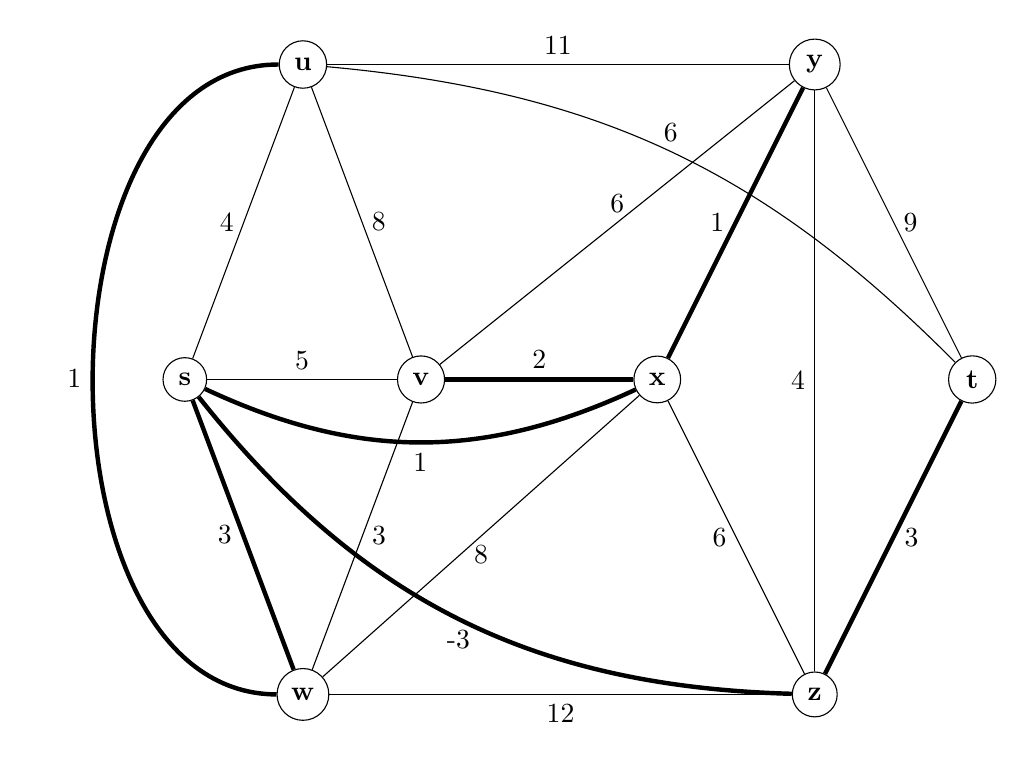
\begin{tikzpicture}
	\node[shape=circle,draw=black] (s) at (1, 4)     {\textbf{s}};
	\node[shape=circle,draw=black] (u) at (2.5, 8)     {\textbf{u}};
	\node[shape=circle,draw=black] (v) at (4, 4)     {\textbf{v}};
	\node[shape=circle,draw=black] (w) at (2.5, 0)     {\textbf{w}};
	\node[shape=circle,draw=black] (x) at (7, 4)     {\textbf{x}};
	\node[shape=circle,draw=black] (y) at (9, 8)     {\textbf{y}};
	\node[shape=circle,draw=black] (z) at (9, 0)     {\textbf{z}};
	\node[shape=circle,draw=black] (t) at (11, 4)     {\textbf{t}};

	\path[-] (s) edge node[left]{4} (u);
	\path[ultra thick] (s) edge [bend right=25] node[below]{-3} (z);
	\path[-] (s) edge node[above]{5} (v);
	\path[ultra thick] (u) edge [bend right=90] node[left]{1} (w);
	\path[-] (u) edge node[above]{11} (y);
	\path[-] (u) edge node[right]{8} (v);
	\path[ultra thick] (s) edge [bend right=25] node[below]{1} (x);
	\path[-] (t) edge [bend right=20] node[above]{6} (u);
	\path[-] (v) edge node[above]{6} (y);
	\path[ultra thick] (v) edge node[above]{2} (x);
	\path[-] (v) edge node[right]{3} (w);
	\path[ultra thick] (w) edge node[left]{3} (s);
	\path[-] (w) edge node[below]{8} (x);
	\path[-] (w) edge node[below]{12} (z);
	\path[ultra thick] (x) edge node[left]{1} (y);
	\path[-] (x) edge node[left]{6} (z);
	\path[-] (y) edge node[left]{4} (z);
	\path[-] (y) edge node[right]{9} (t);
	\path[ultra thick] (z) edge node[right]{3} (t);
		
	\end{tikzpicture} 
	\caption{The minimum spanning tree of Graph G in Q5 after adding (s,z,-3)}
	\label{g9}
\end{figure}

\subsubsection*{Adding (u,y,3)}
\begin{figure}[H]
	\centering
	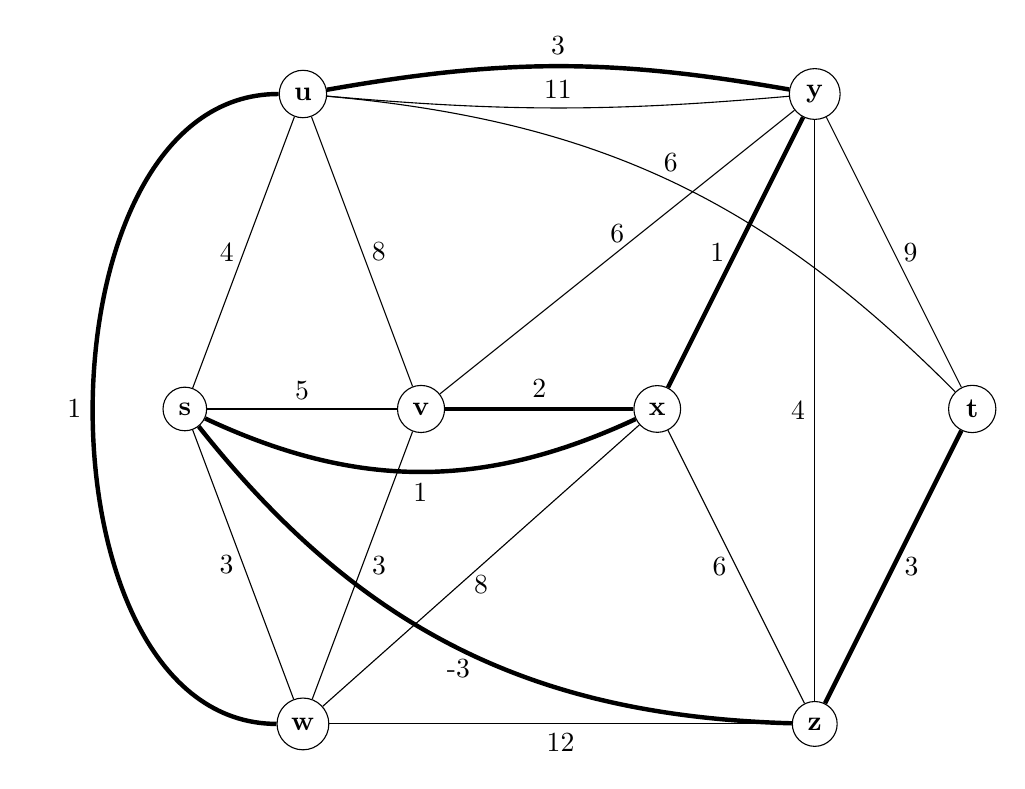
\begin{tikzpicture}
	\node[shape=circle,draw=black] (s) at (1, 4)     {\textbf{s}};
	\node[shape=circle,draw=black] (u) at (2.5, 8)     {\textbf{u}};
	\node[shape=circle,draw=black] (v) at (4, 4)     {\textbf{v}};
	\node[shape=circle,draw=black] (w) at (2.5, 0)     {\textbf{w}};
	\node[shape=circle,draw=black] (x) at (7, 4)     {\textbf{x}};
	\node[shape=circle,draw=black] (y) at (9, 8)     {\textbf{y}};
	\node[shape=circle,draw=black] (z) at (9, 0)     {\textbf{z}};
	\node[shape=circle,draw=black] (t) at (11, 4)     {\textbf{t}};

	\path[-] (s) edge node[left]{4} (u);
	\path[ultra thick] (s) edge [bend right=25] node[below]{-3} (z);
	\path[-] (s) edge node[above]{5} (v);
	\path[ultra thick] (u) edge [bend right=90] node[left]{1} (w);
	\path[ultra thick] (u) edge [bend left=10] node[above]{3} (y);
	\path[-] (u) edge [bend right=5] node[above]{11} (y);
	\path[-] (u) edge node[right]{8} (v);
	\path[ultra thick] (s) edge [bend right=25] node[below]{1} (x);
	\path[-] (t) edge [bend right=20] node[above]{6} (u);
	\path[-] (v) edge node[above]{6} (y);
	\path[ultra thick] (v) edge node[above]{2} (x);
	\path[-] (v) edge node[right]{3} (w);
	\path[-] (w) edge node[left]{3} (s);
	\path[-] (w) edge node[below]{8} (x);
	\path[-] (w) edge node[below]{12} (z);
	\path[ultra thick] (x) edge node[left]{1} (y);
	\path[-] (x) edge node[left]{6} (z);
	\path[-] (y) edge node[left]{4} (z);
	\path[-] (y) edge node[right]{9} (t);
	\path[ultra thick] (z) edge node[right]{3} (t);
		
	\end{tikzpicture} 
	\caption{The minimum spanning tree of Graph G in Q5 after adding (u,y,3)}
	\label{g10}
\end{figure}

\subsubsection*{Adding (w,z,-1)}
\begin{figure}[H]
	\centering
	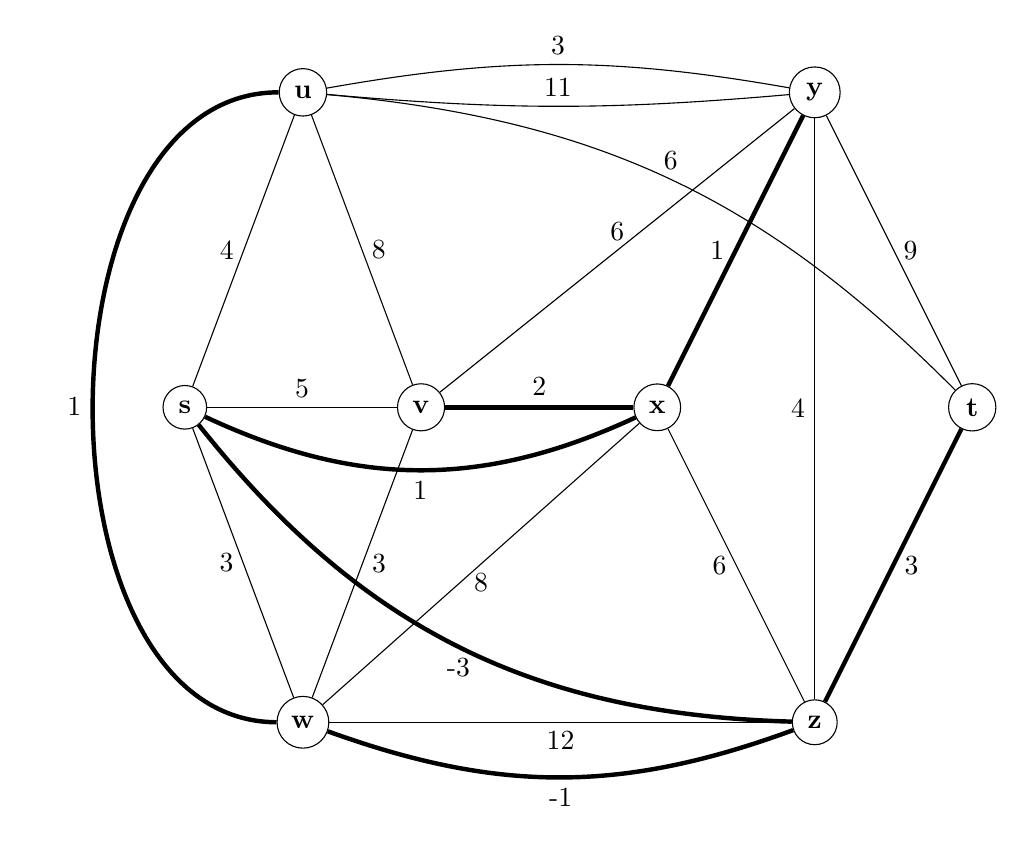
\begin{tikzpicture}
	\node[shape=circle,draw=black] (s) at (1, 4)     {\textbf{s}};
	\node[shape=circle,draw=black] (u) at (2.5, 8)     {\textbf{u}};
	\node[shape=circle,draw=black] (v) at (4, 4)     {\textbf{v}};
	\node[shape=circle,draw=black] (w) at (2.5, 0)     {\textbf{w}};
	\node[shape=circle,draw=black] (x) at (7, 4)     {\textbf{x}};
	\node[shape=circle,draw=black] (y) at (9, 8)     {\textbf{y}};
	\node[shape=circle,draw=black] (z) at (9, 0)     {\textbf{z}};
	\node[shape=circle,draw=black] (t) at (11, 4)     {\textbf{t}};

	\path[-] (s) edge node[left]{4} (u);
	\path[ultra thick] (s) edge [bend right=25] node[below]{-3} (z);
	\path[-] (s) edge node[above]{5} (v);
	\path[ultra thick] (u) edge [bend right=90] node[left]{1} (w);
	\path[-] (u) edge [bend left=10] node[above]{3} (y);
	\path[-] (u) edge [bend right=5] node[above]{11} (y);
	\path[-] (u) edge node[right]{8} (v);
	\path[ultra thick] (s) edge [bend right=25] node[below]{1} (x);
	\path[-] (t) edge [bend right=20] node[above]{6} (u);
	\path[-] (v) edge node[above]{6} (y);
	\path[ultra thick] (v) edge node[above]{2} (x);
	\path[-] (v) edge node[right]{3} (w);
	\path[-] (w) edge node[left]{3} (s);
	\path[-] (w) edge node[below]{8} (x);
	\path[-] (w) edge node[below]{12} (z);
	\path[ultra thick] (w) edge [bend right=20] node[below]{-1} (z);
	\path[ultra thick] (x) edge node[left]{1} (y);
	\path[-] (x) edge node[left]{6} (z);
	\path[-] (y) edge node[left]{4} (z);
	\path[-] (y) edge node[right]{9} (t);
	\path[ultra thick] (z) edge node[right]{3} (t);
		
	\end{tikzpicture} 
	\caption{The minimum spanning tree of Graph G in Q5 after adding (w,z,-1)}
	\label{g11}
\end{figure}

\subsection*{d}
Yes we can update the shortest path without calling \textbf{Dijkstra's Algorithm}. \\
In our initial findings, the shortest path had the following route: $ s \rightarrow v \rightarrow x \rightarrow y \rightarrow z \rightarrow t$, and the cost between each vertex is as follows: $ \{ 5,2,1,4,3 \}$.  If any of the newly added routes includes any of the two points in our initial route, it \textit{may} shorten our path.
\begin{enumerate}
    \item After adding $(s,x,1)$, the distance between $s$ and $x$ shortens, and becomes 1. We can simply update the shortest path cost as $ \{ 1,1,4,3 \}$ with the route $ s  \rightarrow x \rightarrow y \rightarrow z \rightarrow t$, since $s \rightarrow v \rightarrow x$ has a cost of 7, and the newly added edge has a cost of 1. 
    \item After adding $(t,u,6)$, it does not affect any of the routes.
    \item After adding $(s,z,-3)$, the distance between $s$ and $z$ shortens, and becomes -3. We can simply update the shortest path cost as $ \{ -3,3 \}$ with the route $ s  \rightarrow z \rightarrow t$, since $s  \rightarrow x \rightarrow y \rightarrow z $ has a cost of 6, and the newly added edge has a cost of -3. 
    \item After adding $(u,y,3)$, it does not affect any of the routes.
    \item After adding $(w,z,-1)$, it does not affect any of the routes.
\end{enumerate}

\section*{Answer 6}
\subsection*{a}
There are \textbf{13} vertices, \textbf{12} edges on $T$, and it has a height of \textbf{4}.
\subsection*{b}
\texttt{<w:33>,<s:26>,<m:35>,<t:37>,<q:34>,<x:41>,<n:61>,<y:71>,<u:63>,<z:99>,<v:98>,\\ <r:75>,<p:42>}
\subsection*{c}
\texttt{<s:26>,<w:33>,<q:34>,<m:35>,<t:37>,<p:42>,<x:41>,<u:63>,<n:61>,<y:71>,<r:75>,\\<v:98>,<z:99>}
\subsection*{d}
\texttt{<p:42>,<q:34>,<s:26>,<w:33>,<t:37>,<m:35>,<r:75>,<u:63>,<x:41>,<y:71>,<n:61>,\\<v:98>,<z:99>}
\subsection*{e}
\begin{itemize}
    \item  \textbf{Definition 3} from the Section 11.1 of the textbook says that 
    \begin{quote}
        The tree is called a \textit{full m-ary tree} if every internal vertex has exactly $m$ children. An \textit{m-ary} tree with $m$ = 2 is called a binary tree.
    \end{quote}
    \item When we look at $T$, we can see that \texttt{<s:26>,<t:37>,<y:71>,<v:98>} have only 1 children each. Therefore $T$ is not a full binary tree.
\end{itemize}

\subsection*{f}
\begin{itemize}
    \item On a Binary Search Tree, if we do a Inorder Traversal,  since the inorder traversal would follow left-root-right order, and since the left child will always be smaller than the root, similarly the right child will always be greater than the root; we should get ordered keys as the output.
    \item When we take a look at the inorder traversal of $T$, we can see that the pairs \texttt{<p:42>,<x:41>} and  \texttt{<u:63>,<n:61>} are not sorted properly. 
    \item Therefore we can easily say that the given tree $T$ is not a binary search tree.
\end{itemize}

\subsection*{g}
\begin{itemize}
    \item  \textbf{Theorem 5} from the Section 11.1 of the textbook says that 
    \begin{quote}
        There are at most $m^h$ leaves in an m-ary tree of height $h$.
    \end{quote}
    \item Since our tree is 3-ary, and it's a full tree, there must be exactly $3^n$ leaves at height $n$.
    \item If we sum all leaves from $n=0$ to $h$, we would get the following sum;
    $$ \sum\limits_{n=0}^{h}3^n $$ 
    which equals to 
    $$ \sum\limits_{n=0}^{h}3^n = \dfrac{1}{2} \cdot \left( 3^{h+1} - 1 \right)$$ 
\end{itemize}

\subsection*{h}

\begin{figure}[H]
	\centering
	\begin{tikzpicture}
	
	\node[shape=circle,draw=black] (p) at (6, 8)     {\textbf{9}};
	\node[shape=circle,draw=black] (q) at (3, 6)     {\textbf{3}};
	\node[shape=circle,draw=black] (r) at (9.2, 6)     {\textbf{15}};
	
	\node[shape=circle,draw=black] (s) at (1, 4)     {\textbf{1}};
	\node[shape=circle,draw=black] (t) at (5, 4)     {\textbf{7}};
	\node[shape=circle,draw=black] (v) at (11, 4)     {\textbf{22}};
	\node[shape=circle,draw=black] (y) at (7.5, 4)     {\textbf{11}};
	
	\node[shape=circle,draw=black] (m) at (4, 2)     {\textbf{4}};
	\node[shape=circle,draw=black] (z) at (10.2, 2)     {\textbf{21}};

		
	\path[-] (p) edge (q);
	\path[-] (p) edge (r);
	\path[-] (q) edge (t);
	\path[-] (q) edge (s);
	\path[-] (r) edge (v);
	\path[-] (t) edge (m);
	\path[-] (v) edge (z);
	\path[-] (r) edge (y);

	\end{tikzpicture} 
	\caption{Binary Search Tree T with minimum height for Q6.h}	
	\label{bintreeq6}
\end{figure}

\subsection*{i}
\begin{itemize}
    \item Sequence to find 2: \texttt{9} $\xrightarrow{\text{left}}$ \texttt{3} $\xrightarrow{\text{left}}$ \texttt{1} $\xrightarrow{\text{right}}$ \texttt{EMPTY : NOT FOUND} 
    \item Sequence to find 22: \texttt{9} $\xrightarrow{\text{right}}$ \texttt{15} $\xrightarrow{\text{right}}$ \texttt{22 : FOUND}
    
\end{itemize}

\subsection*{j}

\begin{figure}[H]
	\centering
	\begin{tikzpicture}
	
	\node[shape=circle,draw=black] (p) at (2, 8)     {\textbf{0000}};
	\node[shape=circle,draw=black] (q) at (4, 6)     {\textbf{001}};
	\node[shape=circle,draw=black] (r) at (6, 4)     {\textbf{010}};
	\node[shape=circle,draw=black] (s) at (8, 2)     {\textbf{1}};
	\node[shape=circle,draw=black] (t) at (10, 0)     {\textbf{10}};

	\path[-] (p) edge (q);
	\path[-] (q) edge (r);
	\path[-] (r) edge (s);
	\path[-] (t) edge (s);
	
	\end{tikzpicture} 
	\caption{Binary Search Tree T with maximum height for Q6.j}	
	\label{bintreeq62}
\end{figure}

\subsection*{k}

\begin{itemize}
    \item Sequence to find 001: \texttt{0000} $\xrightarrow{\text{right}}$ \texttt{001 : FOUND} 
    \item Sequence to find 011: \texttt{0000} $\xrightarrow{\text{right}}$ \texttt{001} $\xrightarrow{\text{right}}$ \texttt{010} $\xrightarrow{\text{right}}$ \texttt{1} $\xrightarrow{\text{left}}$ \texttt{EMPTY : NOT FOUND}
    
\end{itemize}


\subsection*{l}

\begin{figure}[H]
	\centering
	\begin{tikzpicture}
	
	\node[shape=circle,draw=black] (p) at (6, 8)     {\textbf{g}};
	\node[shape=circle,draw=black] (q) at (3, 6)     {\textbf{f}};
	\node[shape=circle,draw=black] (r) at (9.2, 6)     {\textbf{c}};
	
	\node[shape=circle,draw=black] (s) at (1, 4)     {\textbf{e}};
	\node[shape=circle,draw=black] (t) at (5, 4)     {\textbf{b}};
	
	\node[shape=circle,draw=black] (z) at (14, 8)     {\textbf{a}};

	\node[shape=circle,draw=black] (m) at (4, 2)     {\textbf{d}};
	
		
	\path[-] (p) edge (q);
	\path[-] (p) edge (r);
	\path[-] (q) edge (t);
	\path[-] (q) edge (s);
	\path[-] (t) edge (m);


	\end{tikzpicture} 
	\caption{Spanning Forest for Graph G via Breadth-first Search}	
	\label{bintreeq63}
\end{figure}



\end{document}

​

